\documentclass[aspectratio=169]{beamer}

\usepackage{amsmath}
\usepackage{tikz}
\usepackage{pgfplots}
\usepackage{adjustbox}
\usepackage{hyperref}

\pgfplotsset{compat=1.18}
\usetikzlibrary{positioning, arrows.meta}

\usetheme{Madrid}



\title{Santa's Workshop Tour Optimization}
\author{Deniz Günes, Simão Ribeiro, Sara Ribeiro}

\begin{document}


\frame{\titlepage}


\begin{frame}{1. Problem Definition}

\textbf{Goal:}
\begin{itemize}
    \item Assign each family to a day minimizing total cost
\end{itemize}

\textbf{Objective Function:}
\[
f(S) = \text{Preference Cost} + \text{Accounting Penalty}
\]

\textbf{Hard Constraints:}
\begin{itemize}
    \item Daily occupancy between limits (total number of people attending the workshop each day must be between $125$ and $300$)
\end{itemize}

\textbf{Soft Constraints:}
\begin{itemize}
    \item Family preferences (ranked choices)
\end{itemize}

\end{frame}


\begin{frame}{2. Related Work}

\textbf{Sources Explored:}
\begin{itemize}
    \item Kaggle Leaderboard Solutions
    \item YouTube: Simulated Annealing
\end{itemize}

\vspace{0.3cm}

\textbf{References:}
\begin{itemize}
    \item \href{https://www.kaggle.com/competitions/santa-workshop-tour-2019/writeups/felixoneberlin-how-to-win-santa-s-workshop-tour}{Kaggle Discussion Thread}
    \item \href{https://www.youtube.com/watch?v=klrmv7nuSX4}{Streamlining Scheduling with Simulated Annealing }
\end{itemize}

\vspace{0.3cm}

\textbf{Common Techniques:}
\begin{itemize}
    \item Mixed Integer Linear Programming (most common and winner of the competition)
    \item Simulated Annealing
\end{itemize}

\end{frame}


\begin{frame}{3. Solution Representation}

\textbf{Solution (State):}
\[
S = (d_1, d_2, ..., d_n)
\]

\begin{itemize}
    \item $d_i$ = assigned day for family $i$
\end{itemize}

\vspace{0.3cm}

\textbf{Data Structures (Implementation):}
\begin{itemize}
    \item \textbf{placement\_dict:} family $\rightarrow$ assigned day
    \item \textbf{occupancy\_dict:} day $\rightarrow$ number of people
    \item \textbf{choice\_dict:} family $\rightarrow$ preferred days list
\end{itemize}

\vspace{0.3cm}

\textbf{Initialization:}
\begin{itemize}
    \item Greedy assignment based on preferences
\end{itemize}

\end{frame}


\begin{frame}{4. Neighborhood \& Operators}

\textbf{Neighborhood Function:}
\begin{itemize}
    \item Select a family $i$
    \item Assign a different day from its preference list
\end{itemize}

\[
S' = (d_1, ..., d_i', ..., d_n)
\]

\vspace{0.3cm}

\textbf{Mutation (Simulated Annealing):}
\begin{itemize}
    \item Random reassignment of one family
\end{itemize}

\vspace{0.3cm}

\textbf{Crossover (Not Used):}
\begin{itemize}
    \item Not applicable (single-solution metaheuristic)
\end{itemize}

\vspace{0.3cm}

\textbf{Transition Acceptance:}
\[
P = e^{-\Delta / T}
\]

\end{frame}


\begin{frame}{5. State as a Bipartite Graph}

\textbf{State Representation:}
\begin{itemize}
    \item A state is a valid set of edges in a bipartite graph
    \item Left partition: family nodes ($F_1, \ldots, F_n$)
    \item Right partition: day-choice nodes (possible assigned days)
    \item Each family has exactly one selected edge to one day node
\end{itemize}

\begin{columns}[T]

\begin{column}{0.6\textwidth}
\begin{center}
\begin{adjustbox}{max width=\textwidth}
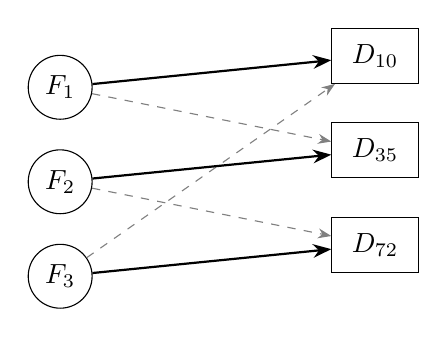
\begin{tikzpicture}[
family/.style={circle, draw, minimum size=7mm},
day/.style={rectangle, draw, minimum width=11mm, minimum height=7mm},
sel/.style={-Stealth, thick},
cand/.style={-Stealth, dashed, gray}
]

\node[family] (F1) at (0,1.2) {$F_1$};
\node[family] (F2) at (0,0) {$F_2$};
\node[family] (F3) at (0,-1.2) {$F_3$};

\node[day] (D10) at (4,1.6) {$D_{10}$};
\node[day] (D35) at (4,0.4) {$D_{35}$};
\node[day] (D72) at (4,-0.8) {$D_{72}$};

\draw[cand] (F1) -- (D35);
\draw[cand] (F2) -- (D72);
\draw[cand] (F3) -- (D10);

\draw[sel] (F1) -- (D10);
\draw[sel] (F2) -- (D35);
\draw[sel] (F3) -- (D72);

\end{tikzpicture}
\end{adjustbox}
\end{center}
\end{column}

\begin{column}{0.4\textwidth}
\textbf{Interpretation:}
\begin{itemize}
    \item Solid edges = chosen assignments defining the state
    \item Dashed edges = alternative candidate assignments
    \item Validity requires occupancy constraints on each day
\end{itemize}
\end{column}

\end{columns}

\end{frame}


\begin{frame}{6. Evaluation Function}

\textbf{Total Cost:}
\[
f(S) = C_{pref} + C_{account}
\]

\vspace{0.3cm}

\textbf{Preference Cost:}
\begin{itemize}
    \item Santa provides consolation gifts according to each family's assigned day relative to their preference rank
    \item The sum of these gifts over all families is the preference cost ($C_{pref}$)
    \item choice\_0: no consolation gifts
    \item choice\_1: one \$50 gift card to Santa's Gift Shop
    \item choice\_2: one \$50 gift card, and 25\% off Santa's Buffet (value \$9) for each family member
    \item choice\_3: one \$100 gift card, and 25\% off Santa's Buffet (value \$9) for each family member
    \item choice\_4: one \$200 gift card, and 25\% off Santa's Buffet (value \$9) for each family member
\end{itemize}

\end{frame}


\begin{frame}{6. Evaluation Function (cont.)}

\begin{itemize}
    \item choice\_5: one \$200 gift card, and 50\% off Santa's Buffet (value \$18) for each family member
    \item choice\_6: one \$300 gift card, and 50\% off Santa's Buffet (value \$18) for each family member
    \item choice\_7: one \$300 gift card, and free Santa's Buffet (value \$36) for each family member
    \item choice\_8: one \$400 gift card, and free Santa's Buffet (value \$36) for each family member
    \item choice\_9: one \$500 gift card, and free Santa's Buffet (value \$36) for each family member, and 50\% off North Pole Helicopter Ride tickets (value \$199) for each family member
    \item otherwise: one \$500 gift card, and free Santa's Buffet (value \$36) for each family member, and free North Pole Helicopter Ride tickets (value \$398) for each family member
\end{itemize}

\end{frame}


\begin{frame}{6. Evaluation Function (cont.)}
\textbf{Accounting Penalty:}
\begin{itemize}
    \item Extra empirical cost based on occupancy and day-to-day variation:
\[
\sum_{d=100}^{1} \frac{N_d - 125}{400} N_d^{\left(0.5 + \frac{|N_d - N_{d+1}|}{50}\right)}
\]
    \item Where $N_d$ is occupancy on day $d$, $N_{d+1}$ is occupancy on the previous day, and for $d=100$, $N_{101}=N_{100}$
\end{itemize}
\vspace{0.3cm}
\textbf{Hard Constraint Handling:}
\begin{itemize}
    \item Invalid states are rejected
     \begin{itemize}
        \item The total number of people attending the workshop each day must be between 125 and 300
     \end{itemize}
\end{itemize}

\vspace{0.3cm}

\end{frame}


\begin{frame}{7. Simulated Annealing Behavior}

\begin{center}
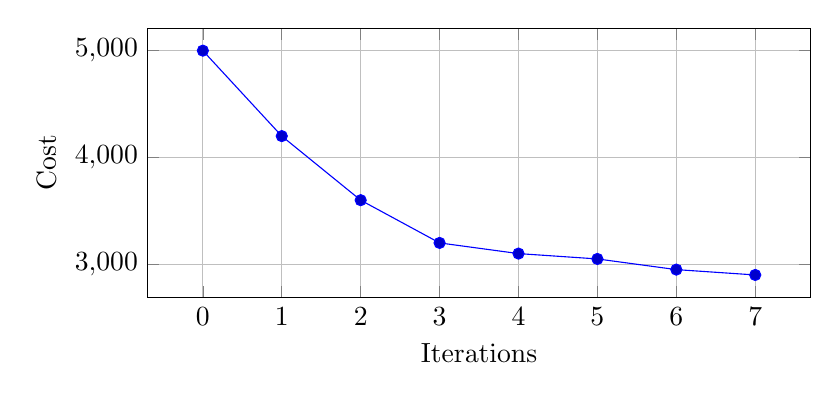
\begin{tikzpicture}
\begin{axis}[
    width=10cm,
    height=5cm,
    xlabel=Iterations,
    ylabel=Cost,
    grid=major
]

\addplot coordinates {
(0,5000) (1,4200) (2,3600) (3,3200)
(4,3100) (5,3050) (6,2950) (7,2900)
};

\end{axis}
\end{tikzpicture}
\end{center}

\vspace{0.2cm}

\textbf{Behavior:}
\begin{itemize}
    \item Early exploration (high temperature)
    \item Later exploitation (low temperature)
\end{itemize}

\end{frame}


\begin{frame}{8. Implementation}

\textbf{Technology:}
\begin{itemize}
    \item Python + Pandas
\end{itemize}

\textbf{Approach:}
\begin{itemize}
    \item Greedy initialization
    \item Iterative Simulated Annealing loops
\end{itemize}

\vspace{0.3cm}

\textbf{Key Features:}
\begin{itemize}
    \item Efficient cost recomputation
    \item Dictionary-based state tracking
\end{itemize}

\vspace{0.3cm}

\textbf{Next Steps:}
\begin{itemize}
    \item Tune cooling schedule
    \item Improve neighborhood selection
    \item Try ILP formulation and MILP solvers
\end{itemize}

\end{frame}



\end{document}